\chapter{Implementing the System: The Back-End}
	In chapter \ref{chap:design} the design of the solution was described. This description ranged from overall specifications, to more detailed model designs. In the following two chapters the implementation of a \emph{prototype}, following the design specifications from chapter \ref{chap:design}, is described.

	To achieve the best possibly experience for the reader, the description is split into two parts: The back-end and the front-end. In \emph{this} chapter, the implemenation of the prototype back-end is described.


	\section{The Language of the Back-End}
		\subsection{Python}
			One of the more popular languages for self-hosted software is Python. Combined with frameworks such as Django or Flask, it acts as a very powerful way to develop a web API.




		\subsection{Ruby}
		\subsection{Node.js}
		\subsection{C\#}
		\subsection{PHP}
		\subsection{C++}

	\section{To Framework or Not To Framework}
		\subsection{Express}
		\subsection{Hapi}
		\subsection{Restify}
		\subsection{Koa}


	\section{Database Abstraction Layer}
		As decided in section \ref{sec:restrict:database} on page \pageref{sec:restrict:database}, a database abstraction layer is necessary. While Object-Relational Mapping \emph{(ORM)} strictly speaking isn't the same as a DAL, for this section the two are considered equivalent.

		The two most widely used solutions for this, is Sequelize, Bookshelf, and Knex \emph{(Bookshelf is built ontop of Knex)}. Sequelize and Bookshelf are both ORMs, whereas Knex is a DAL. In regards to platform support, they are fairly similar. Sequelize supports PostgreSQL, MySQL, SQLite and MSSQL. Bookshelf/Knex supports MySQL, SQLite, Postgres, MariaDB, and Oracle.

		While working with ORMs generally takes database interactions to a higher abstraction level, it is thought that this also removes certain insight into how some queries work. Additionally, Knex's chainable methods, makes for query building in the style of Javascript promises. As such, it is concluded the Knex is the superior choice as a DAL for the implementation.

	\section{API Endpoints}
		\label{sec:api}
		Before defining the endpoints, the resources \emph{(see section \ref{sec:design:rest} on page \pageref{sec:design:rest})} of the application need to be determined. Looking at the models defined in section \ref{sec:modelling} on page \pageref{sec:modelling}, these offer a great starting point for resources.


		\subsection{The Users Resource}
			First and foremost there is the collection of Users. This collections represents the user base as a whole. \verb=POST=ing to this collection, would by extension mean the creation of a new user. \verb=GET=ing the user collection, mean retrieving all user entries, with their username and other attributes in the ``public domain''. \verb=PUT= and \verb=DELETE= is slightly different. They're used for updating and deleting a \emph{single} user, in the entire collection. As such, the endpoint needs to have a user ID postfixed. Adhering to the standard, \emph{all} API endpoints will have \verb=/api= prefixed. These API endpoints are listed on table \ref{tab:api:users} on page \pageref{tab:api:users}.

		\subsection{The Passwords Resource}
			Then there is the collection of passwords. However, there is a slight caveat when it comes to this collection. Since each password is \emph{owned} by a user, it can generally be thought that there exists \emph{multiple} collection -- one for each user. As such, the password collection is gated behind the user resource and the ID specifying exactly which user owns said password. The same approach to designing these endpoints are used, as with the user resource and the result of this is found on table \ref{tab:api:passwords} on page \pageref{tab:api:passwords}.

			For simplicity's sake, access to shared passwords are gated behind the passwords resource. As such, a collection called shares -- which belongs to a specific password -- denotes the collection of users this specific password has been shared to. Additionally, two collections are added as well: \verb=shared= and \verb=shares=. These two are  \emph{very} similar in name, which unfortunately might result in some confusion. The \verb=shares= resource denotes passwords shared \emph{to} the user and the \verb=shared= resource denotes passwords that the user has shared to \emph{others}. These endpoints are found on table \ref{tab:api:sharedpasswords} on page \pageref{tab:api:sharedpasswords}.

		\subsection{The Categories Resource}
			The same argument made in regards to the passwords collection, can be said about categories. Each user has their own private password collection, which is -- similar to passwords -- gated behind the owning user's ID. This can be seen on table \ref{tab:api:categories} on page \pageref{tab:api:categories}.

		\subsection{The Invites Resource}
			When an admin creates a new invites, it can be said he \verb=POST=s it to the invites resource. \verb=GET=ing an ID, returns the status of an ID stored in the database. Then, there is finally the act of using an invite. Since a user is created, it only makes sense that the \verb=POST= method is needed. However, since the regular endpoint is already being posted to, an additional endpoint is needed. As such, appending the endpoint with \verb=/accept= will achieve this. This can be seen on table \ref{tab:api:invites} on page \pageref{tab:api:invites}.

		\subsection{The Audit Resource}
			The Audit resource is actually very simple. It only consists of a single endpoint; Getting the audit log. Since this resource is owned by individual users, this is -- much like passwords and categories -- gated behind the user collection and a specific ID. This can be seen on table \ref{tab:api:audit} on page \pageref{tab:api:audit}.

		\subsection{The Auth Resource}
			\label{sec:api:auth}
			The Auth resource is a little bit more interesting. Of course, there is the generic \verb=POST=, containing the user's username and password, for authentication purposes. The details of this is covered in section \ref{sec:design:authentication} on page \pageref{sec:design:authentication}. However, this is not all. Since the solution supports TOTP two-factor-authentication, as described in section \ref{sec:mfa} on page \pageref{sec:mfa}, endpoints for enabling this is needed as well. In section \ref{sec:design:breaking-rest} on page \pageref{sec:design:breaking-rest} it was argued that at one point it was \emph{necessary} to break the REST principles. As such, two endpoints are needed: One for generating a new secret and caching it, and one for actually verifying said secret. 


		
		\newcolumntype{L}[1]{>{\hsize=#1\hsize\raggedright\arraybackslash}X}%
		\newcolumntype{R}[1]{>{\hsize=#1\hsize\raggedleft\arraybackslash}X}%
		\newcolumntype{C}[2]{>{\hsize=#1\hsize\columncolor{#2}\centering\arraybackslash}X}%
		
		\begin{table}
			\definecolor{tablerow1}{RGB}{230,230,230}
			\definecolor{tablerow2}{RGB}{255,255,255}
			\rowcolors{2}{tablerow1}{tablerow2}
			
			\begin{tabularx}{\textwidth}{ R{0.2} | L{0.6} | L{0.2} }
				\bfseries Method & \bfseries Endpoint & \bfseries Description% specify table head
				\csvreader[head to column names]{resources/api/users.csv}{}% use head of csv as column names
				{\\\hline\method & \texttt{\endpoint} & \description}% specify your coloumns here
			\end{tabularx}

			\caption{API endpoints for the Users resource.}
			\label{tab:api:users}
		\end{table}


		\begin{table}
			\definecolor{tablerow1}{RGB}{230,230,230}
			\definecolor{tablerow2}{RGB}{255,255,255}
			\rowcolors{2}{tablerow1}{tablerow2}
			
			\begin{tabularx}{\textwidth}{ R{0.2} | L{0.6} | L{0.2} }
				\bfseries Method & \bfseries Endpoint & \bfseries Description% specify table head
				\csvreader[head to column names]{resources/api/passwords.csv}{}% use head of csv as column names
				{\\\hline\method & \texttt{\endpoint} & \description}% specify your coloumns here
			\end{tabularx}

			\caption{API endpoints for the Passwords resource.}
			\label{tab:api:passwords}
		\end{table}

		\begin{table}
			\definecolor{tablerow1}{RGB}{230,230,230}
			\definecolor{tablerow2}{RGB}{255,255,255}
			\rowcolors{2}{tablerow1}{tablerow2}
			
			\begin{tabularx}{\textwidth}{ R{0.2} | L{0.6} | L{0.2} }
				\bfseries Method & \bfseries Endpoint & \bfseries Description% specify table head
				\csvreader[head to column names]{resources/api/sharedPasswords.csv}{}% use head of csv as column names
				{\\\hline\method & \texttt{\endpoint} & \description}% specify your coloumns here
			\end{tabularx}

			\caption{API endpoints for accessing Shared Passwords.}
			\label{tab:api:sharedpasswords}
		\end{table}		

		\begin{table}
			\definecolor{tablerow1}{RGB}{230,230,230}
			\definecolor{tablerow2}{RGB}{255,255,255}
			\rowcolors{2}{tablerow1}{tablerow2}
			
			\begin{tabularx}{\textwidth}{ R{0.2} | L{0.6} | L{0.2} }
				\bfseries Method & \bfseries Endpoint & \bfseries Description% specify table head
				\csvreader[head to column names]{resources/api/categories.csv}{}% use head of csv as column names
				{\\\hline\method & \texttt{\endpoint} & \description}% specify your coloumns here
			\end{tabularx}

			\caption{API endpoints for the Categories resource.}
			\label{tab:api:categories}
		\end{table}
		
		\begin{table}
			\definecolor{tablerow1}{RGB}{230,230,230}
			\definecolor{tablerow2}{RGB}{255,255,255}
			\rowcolors{2}{tablerow1}{tablerow2}
			
			\begin{tabularx}{\textwidth}{ R{0.2} | L{0.6} | L{0.2} }
				\bfseries Method & \bfseries Endpoint & \bfseries Description% specify table head
				\csvreader[head to column names]{resources/api/invites.csv}{}% use head of csv as column names
				{\\\hline\method & \texttt{\endpoint} & \description}% specify your coloumns here
			\end{tabularx}

			\caption{API endpoints for the Invites resource.}
			\label{tab:api:invites}
		\end{table}

		\begin{table}
			\definecolor{tablerow1}{RGB}{230,230,230}
			\definecolor{tablerow2}{RGB}{255,255,255}
			\rowcolors{2}{tablerow1}{tablerow2}
			
			\begin{tabularx}{\textwidth}{ R{0.2} | L{0.6} | L{0.2} }
				\bfseries Method & \bfseries Endpoint & \bfseries Description% specify table head
				\csvreader[head to column names]{resources/api/audit.csv}{}% use head of csv as column names
				{\\\hline\method & \texttt{\endpoint} & \description}% specify your coloumns here
			\end{tabularx}

			\caption{API endpoint for the Audit resource.}
			\label{tab:api:audit}
		\end{table}

		\begin{table}[p]
			\definecolor{tablerow1}{RGB}{230,230,230}
			\definecolor{tablerow2}{RGB}{255,255,255}
			\rowcolors{2}{tablerow1}{tablerow2}
			
			\begin{tabularx}{\textwidth}{ R{0.2} | L{0.6} | L{0.2} }
				\bfseries Method & \bfseries Endpoint & \bfseries Description% specify table head
				\csvreader[head to column names]{resources/api/auth.csv}{}% use head of csv as column names
				{\\\hline\method & \texttt{\endpoint} & \description}% specify your coloumns here
			\end{tabularx}

			\caption{API endpoints for the Auth resource.}
			\label{tab:api:auth}
		\end{table}

	\section{Workaround To Be Self-Contained}
		Unfortunatly, Restify's documentation is sometimes lackluster. They have what they call the serveStatic method. From their decription, its intended use is to deliver a default file, if a match is not found. This is exactly what is needed for the front-end's router \emph{(more on this in section \ref{sec:impl:ui-router} on page \pageref{sec:impl:ui-router})}. However, after much fiddling, it was found simply not to work.

		As such, a workaround is needed. After having stated the API routes, six new routes are defined as is seen on table \ref{tab:api:workaround} on page \pageref{tab:api:workaround}. This ensures that any API hits are given the proper error code, while ensuring that the application for the front-end is being delivered in all cases.
		\begin{table}
			\centering
			\begin{tabular}{r | l}
				\textbf{Method} & \textbf{Endpoint} \\
				\hline
				\verb=GET=		& \verb=/api/.*= \\
				\verb=HEAD=		& \verb=/api/.*= \\	
				\verb=POST=		& \verb=/api/.*= \\	
				\verb=PUT=		& \verb=/api/.*= \\
				\verb=DEL=		& \verb=/api/.*= \\
				\verb=PATCH=	& \verb=/api/.*= \\	
			\end{tabular}
			\caption{Workaround error routes, to make the API adhere to standards and the front-end's router to work \emph{(see section \ref{sec:impl:ui-router} on page \pageref{sec:impl:ui-router})}}
			\label{tab:api:workaround}
		\end{table}
		%RESTIFY workaround with serve static

	\section{Authentication}
		In section \ref{sec:api:auth} on page \pageref{sec:api:auth} the endpoints involved in authentication was described. In this section, the process is described a little further. 

		As with any authentication, the user starts by sending his or her username and password \emph{(see section \ref{sec:design:authentication} on page \pageref{sec:design:authentication})}. If two factor authentication is not enabled, the standard verification approach is made. If the password matches, http code \verb=200= is returned, signifying successful authentication. Should it not match, http code \verb=401= is returned, signifying unsuccessful authentication. All in all, very basic.

		Should two factor authentication be enabled, however, a more complex event happens. Since the front-end won't know if two factor authentication is enabled or not, this needs to be conveyed to the front-end. As such, should the user have two-factor authentication enabled, but the token is missing from the body, http error code \verb=403= is returned. \verb=403= is defined as follows, by RFC2616\cite{httpcodes}:
		\begin{citequote}[sec.10.4.4]{httpcodes}
			   The server understood the request, but is refusing to fulfill it...
		\end{citequote}
		When the front-end receives the \verb=403= from the authentication endpoint, it \emph{knows} to promt to the user for a two-factor-token. Once this token is obtained, the request is sent again -- with the new token. Once received, the back-end verifies the password, similar to before, and verifies that the token is correct. If all fields are vitrified the back-end responds with \verb=200= to signify successful authentication. Should both fields not be verified, the response is \verb=401= to signify unsuccessful authentication. Figure \ref{fig:sequence:auth} on page \pageref{fig:sequence:auth} depicts this series of event, in a sequence diagram.

		\begin{figure}[p]
			\centering
			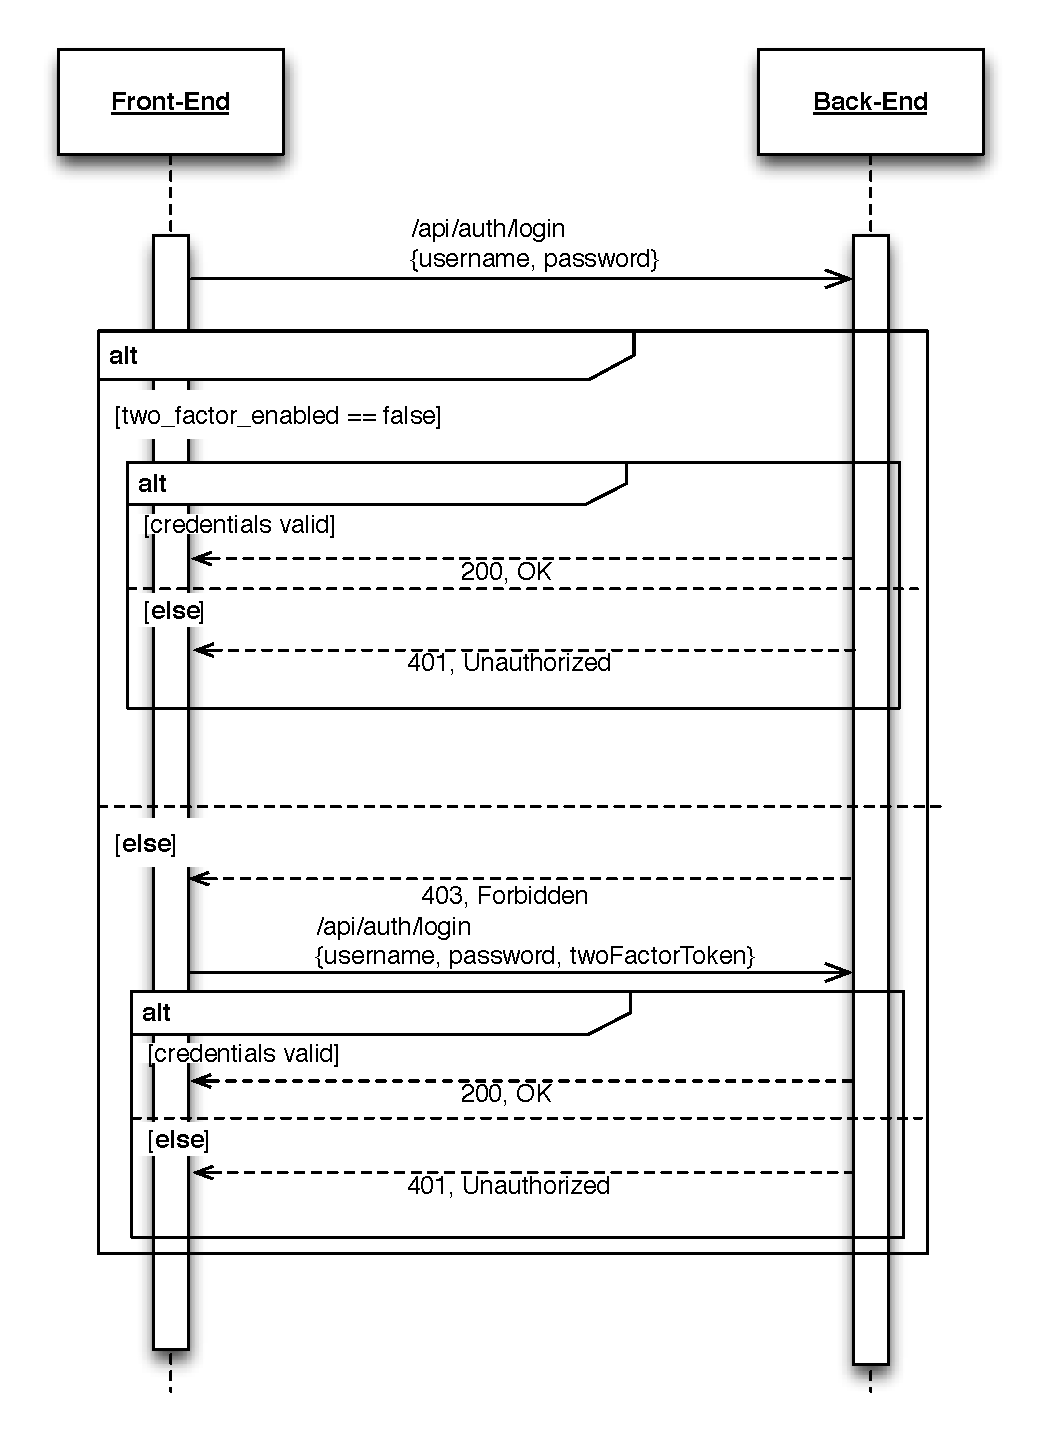
\includegraphics[width=0.8\textwidth]{figures/implementation/uml/sequence/authentication.eps}
			\caption{Sequence diagram showing the process of how the front-end authenticates to the back-end.}
			\label{fig:sequence:auth}
		\end{figure}

	\section{Authorization}
		For authorization purposes two strategies will be used: Simple and advanced. For all purposes where the simple is a possibility, it will be used. In section \ref{sec:design:authorization} on page \pageref{sec:design:authorization} it was described which users has access to which entities. The following two sections will adhere to this design.

		\subsection{Basic Authorization}
			Using the API described in section \ref{sec:api} on page \pageref{sec:api}, it is clearly seen that models' IDs are found in the URL. As such, using the owner field, of these models, it can easily be determined if the authenticated user has access to any given resource.

			As per the design, \emph{both} the user and admins will have full access to all user methods. This is simply handled with a comparison:
			\begin{lstlisting}[gobble=16,language=JavaScript]
                if( req.resolved.user.id === user.id || req.resolved.user.isAdmin ){
			\end{lstlisting}

			Since it is only the user self, that has access to his or her passwords, this is also handled extremely easy by doing:
			\begin{lstlisting}[gobble=16,language=JavaScript]
                if( password.owner === user.id && user.id === req.resolved.user.id ){
			\end{lstlisting}
			The exact same is done for categories:
			\begin{lstlisting}[gobble=16,language=JavaScript]
                if( category.owner === user.id && user.id === req.resolved.user.id ){
			\end{lstlisting}

			Shared passwords however, are a little bit more difficult. As has already been stated, both the user \emph{sharing} the password and the user receiving the shared password needs access to this resource. As such, the logic is a little different:
			\begin{lstlisting}[gobble=16,language=JavaScript]
                if( (share.owner === user.id && user.id === req.resolved.user) || (share.origin_owner === user.id && user.id === req.resolved.user)){
			\end{lstlisting}
		
			If the above snippets are evaluated to \verb=true=, the code keeps executing. If it is evaluated to false, the back-end returns http code \verb=403=, Forbidden denoting that the user does \emph{not} have sufficient privileges to access that specific data.

		\subsection{Advanced Authentication}
			However, this only works on select resources. As the user will easily see, the invite endpoints will not work using the simple method. As such, the groundwork for a more advanced and fine grained authorization framework is made.

			First and foremost, the basic target is defined. In this case, it will be \verb=invite=. Next, the actions on this target is defined. For invites, there really only is one: \verb=create=. For other objects, these actions might be \verb=update=, \verb=delete=, etc. Then, for each target, each method's permissions can be defined. In the invites case, the following snippet shows the authorization process:

			\begin{lstlisting}[gobble=16,language=JavaScript]
                function invite(permObject, req, res, next){
                    // Supported Methods
                    var methods = ['create'];
                    
                    // Check to see if method is supported in authorization suite
                    if( _.indexOf(methods, permObject.method) === -1 ){
                        return deny(next);
                    }
                    
                    if( permObject.method === methods[0] ){
                        // Allow creation of invite, if the user is an admin
                        if( req.resolved.user.isAdmin ){
                            return next();
                        }

                        return next(new restify.errors.ForbiddenError('Insufficient privileges'));
                    }
                }			
			\end{lstlisting}
			The \verb=deny(..)= method is just a wrapper to elegantly throw the same error, across multiple authorization targets. The content of this method is as simple as:
			\begin{lstlisting}[gobble=16,language=JavaScript]
                function deny(next){
                    return next(new restify.errors.ForbiddenError('Insufficient privileges'));
                }
			\end{lstlisting}

		\subsection{Simple or Advanced}
			There is not a seconds doubt that the advanced approach is more fine grained. Where the simple approach only supports differentiating between targets, the advanced approach also supports differentiating between actions. As such, while the simple method does its job perfectly as is, should the need for more detailed authorization options arise, they will need to be implemented the advanced approach.


	\section{Dependencies}


\chapter{Implementing the System: The Front-End}
	\section{Developing for the Browser}
		\subsection{Flash}
		\subsection{Java}
		\subsection{Javascript}
		\subsection{Silverlight}


	\section{Using a Framework}
		\begin{itemize}
			\item Angular 1.5
			\item Angular 2.0
			\item ReactJS
			\item Ember
			\item Polymer
		\end{itemize}


	\section{UI-Router}
		\label{sec:impl:ui-router}

	\section{Performing Encryption}

	\section{Generating Passwords}


	
	\section{Resolving Objects}
		restify middelware automaticly get objects from storage
